\documentclass[12pt,a4paper]{article}

\usepackage[a4paper, margin=1in]{geometry}
\usepackage{graphicx}
\usepackage{booktabs}
\usepackage{array}
\usepackage{longtable}
\usepackage{tabularx}
\usepackage{xcolor}
\usepackage{colortbl}
\usepackage{fancyhdr}
\usepackage{titlesec}
\usepackage{enumitem}
\usepackage{hyperref}
\usepackage[T1]{fontenc}
\usepackage[utf8]{inputenc}
\usepackage{parskip}
\usepackage{amsmath}
\setlength{\headheight}{14pt}
\usepackage{multirow}
\usepackage{makecell}
\usepackage{lastpage}
\usepackage{float}

\graphicspath{{images/}}

\definecolor{darkblue}{RGB}{31,56,100}
\definecolor{medblue}{RGB}{46,80,144}
\definecolor{tableheadbg}{RGB}{31,56,100}
\definecolor{rowaltbg}{RGB}{238,242,248}
\definecolor{hred}{RGB}{192,0,0}
\definecolor{mred}{RGB}{127,127,0}
\definecolor{gray}{RGB}{136,136,136}

\hypersetup{
    colorlinks=true,
    linkcolor=medblue,
    urlcolor=medblue,
    pdftitle={SA/SD - Hotel Automation Software v1.0},
    pdfauthor={Project Team}
}

\titleformat{\section}
  {\Large\bfseries\color{darkblue}}
  {\thesection}{1em}{}
  [\vspace{2pt}\color{medblue}\titlerule[1pt]\vspace{4pt}]
\titleformat{\subsection}
  {\large\bfseries\color{medblue}}
  {\thesubsection}{1em}{}
\titleformat{\subsubsection}
  {\normalsize\bfseries\color{medblue}}
  {\thesubsubsection}{1em}{}

\pagestyle{fancy}
\fancyhf{}
\fancyhead[L]{\small\color{medblue} Structured Analysis \& Structured Design}
\fancyhead[R]{\small\color{gray} Hotel Automation Software}
\fancyfoot[L]{\small\color{gray} Version 1.0 \textbar\ Confidential}
\fancyfoot[R]{\small\color{gray} Page \thepage\ of \pageref{LastPage}}
\renewcommand{\headrulewidth}{0.5pt}
\renewcommand{\footrulewidth}{0.5pt}

\newcolumntype{L}[1]{>{\raggedright\arraybackslash}p{#1}}
\newcolumntype{C}[1]{>{\centering\arraybackslash}p{#1}}
\newcolumntype{R}[1]{>{\raggedleft\arraybackslash}p{#1}}

\renewcommand{\thead}[1]{%
  \cellcolor{tableheadbg}\color{white}\textbf{#1}%
}

\begin{document}

% ── COVER PAGE ────────────────────────────────────────────────────────────────
\thispagestyle{empty}
\begin{center}
  \vspace*{3cm}
  {\Huge\bfseries\color{darkblue} STRUCTURED ANALYSIS\\[0.3em] \&\\[0.3em] STRUCTURED DESIGN}\\[1em]
  {\LARGE\color{medblue} Hotel Automation Software}\\[3cm]

  \begin{tabular}{|L{4cm}|L{8cm}|}
    \hline
    \rowcolor{tableheadbg}
    \color{white}\textbf{Document Type} & \color{white} Structured Analysis \& Structured Design (SA/SD) \\
    \hline
    \rowcolor{rowaltbg}
    \textbf{Subject}           & Software Engineering \\
    \hline
    \rowcolor{rowaltbg}
    \textbf{Subject Code}      & CS3004 \\
    \hline
    \textbf{Version}           & 1.0 (PlantUML-rendered diagrams) \\
    \hline
    \rowcolor{rowaltbg}
    \textbf{Date}              & \today \\
    \hline
    \rowcolor{rowaltbg}
    \textbf{Based on SRS}      & SRS\_HotelAutomation\_v1.0 \\
    \hline
   \textbf{Group Members}     &
      \begin{tabular}[t]{@{}L{4cm} L{3.5cm}@{}}
        Suyash Pandey        & : 2023UG1100 \\[3pt]
        Suraj Kumar          & : 2023UG1106 \\[3pt]
        Himanshu Raj          & : 2023UG1092 \\[3pt]
        Satyendra Kumar         & : 2023UG1105 \\
      \end{tabular} \\
    \hline
    \rowcolor{rowaltbg}
    \textbf{Institution}       & Indian Institute of Information Technology Ranchi, Jharkhand \\
    \hline
  \end{tabular}
\end{center}
\vfill
\begin{center}
  \color{gray}\small\textit{Copying of assignments is considered a serious offense.}
\end{center}
\newpage

% ── TABLE OF CONTENTS ─────────────────────────────────────────────────────────
\thispagestyle{fancy}
\tableofcontents
\newpage

% ══════════════════════════════════════════════════════════════════════════════
\section{Introduction}

\subsection{Purpose}

This document presents the Structured Analysis (SA) and Structured Design (SD) for the
\textbf{Hotel Automation Software}. It decomposes the system defined in the Software
Requirements Specification (SRS v1.0) into data-flow diagrams (DFDs), a data
dictionary, a structure chart, and module specifications suitable for direct
implementation in Java / Java Swing backed by an embedded relational database.

\subsection{Notation}

\textbf{DFD notation}:
\begin{itemize}[leftmargin=1.5em]
  \item \textbf{Process} --- blue ellipse, labelled \texttt{n.m Name}.
  \item \textbf{External entity} --- orange rectangle.
  \item \textbf{Data store} --- green cylinder, labelled \texttt{Dn Name}.
  \item \textbf{Data flow} --- directed arrow with a data-name label.
\end{itemize}
(PlantUML renders data stores as cylinders rather than the classical open-rectangle;
the semantics are identical.)

\noindent\textbf{Structure-chart notation}:
\begin{itemize}[leftmargin=1.5em]
  \item \textbf{Module} --- rectangle labelled with the module name.
  \item \textbf{Call} --- arrow from caller to callee.
  \item Data and flag couples are listed in Table~\ref{tbl:couples} rather than on the
        diagram itself, to keep the layout readable.
\end{itemize}

\subsection{Diagram Toolchain}

Diagrams are authored in \textbf{PlantUML} (source in \texttt{puml/}) and rendered to
PNG via the PlantUML online editor or a local \texttt{plantuml.jar}. The PNGs live in
\texttt{images/} and are embedded below via \verb|\includegraphics|. See
\texttt{SA\_SD/README.md} for rendering instructions.

\subsection{Traceability}

Every process in the DFDs and every module in the structure chart is cross-referenced
to the SRS requirements it realises. A consolidated traceability matrix appears in
Section~\ref{sec:trace}.

\newpage

% ══════════════════════════════════════════════════════════════════════════════
\section{Structured Analysis}

\subsection{Context Diagram (Level 0)}

The Level-0 (context) DFD treats the entire system as a single process and shows only
its interactions with external entities.

\begin{figure}[H]
\centering
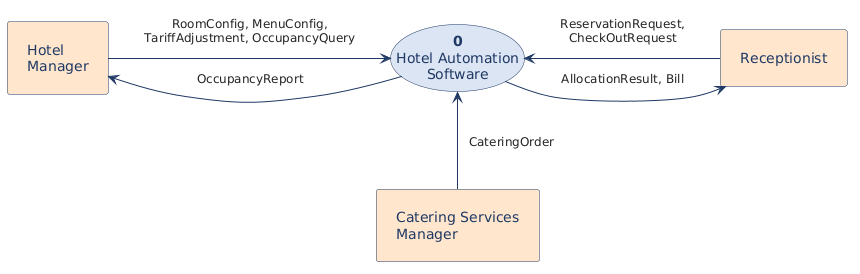
\includegraphics[width=0.75\textwidth,keepaspectratio]{context.png}
\caption{Context Diagram (Level 0)}
\label{fig:level0}
\end{figure}

\noindent\textbf{External entities.} The system interacts with four distinct external
entities corresponding to the user classes defined in SRS~\S2.3:

\begin{itemize}[leftmargin=1.5em]
  \item \textbf{Hotel Manager} --- configures rooms, tariffs, food menu, and discount
        policies; reviews occupancy reports.
  \item \textbf{Receptionist} --- manages guest reservations, room allocations, token
        issuance, and check-out.
  \item \textbf{Catering Services Manager} --- records food and beverage orders against
        guest token numbers.
  \item \textbf{Guest} --- the indirect beneficiary; interacts via the Receptionist and
        Catering Services Manager.
\end{itemize}

\noindent\textbf{Data flows.}
\begin{itemize}[leftmargin=1.5em]
  \item \textbf{RoomConfig} --- room numbers, bed types, AC types, and initial tariffs
        supplied by the Hotel Manager.
  \item \textbf{TariffAdjustment} --- room type and percentage adjustment value supplied
        by the Hotel Manager.
  \item \textbf{OccupancyQuery} --- month selection from the Hotel Manager; system
        returns \textbf{OccupancyReport}.
  \item \textbf{MenuConfig} --- food item names and unit prices supplied by the Hotel
        Manager.
  \item \textbf{ReservationRequest} --- guest name, arrival date/time, duration, room
        type preference, advance payment, optional frequent-guest identity number, supplied
        by the Receptionist.
  \item \textbf{AllocationResult} --- room number and token number (success) or apology
        message (failure) returned to the Receptionist.
  \item \textbf{CateringOrder} --- token number, food item, quantity, date and time
        supplied by the Catering Services Manager.
  \item \textbf{CheckOutRequest} --- token number supplied by the Receptionist to
        initiate billing.
  \item \textbf{Bill} --- itemised bill with net balance payable, returned to the
        Receptionist for printing.
\end{itemize}

\newpage

\subsection{Level-1 DFD}

Process~0 is decomposed into six cooperating processes and six data stores.

\begin{figure}[H]
\centering
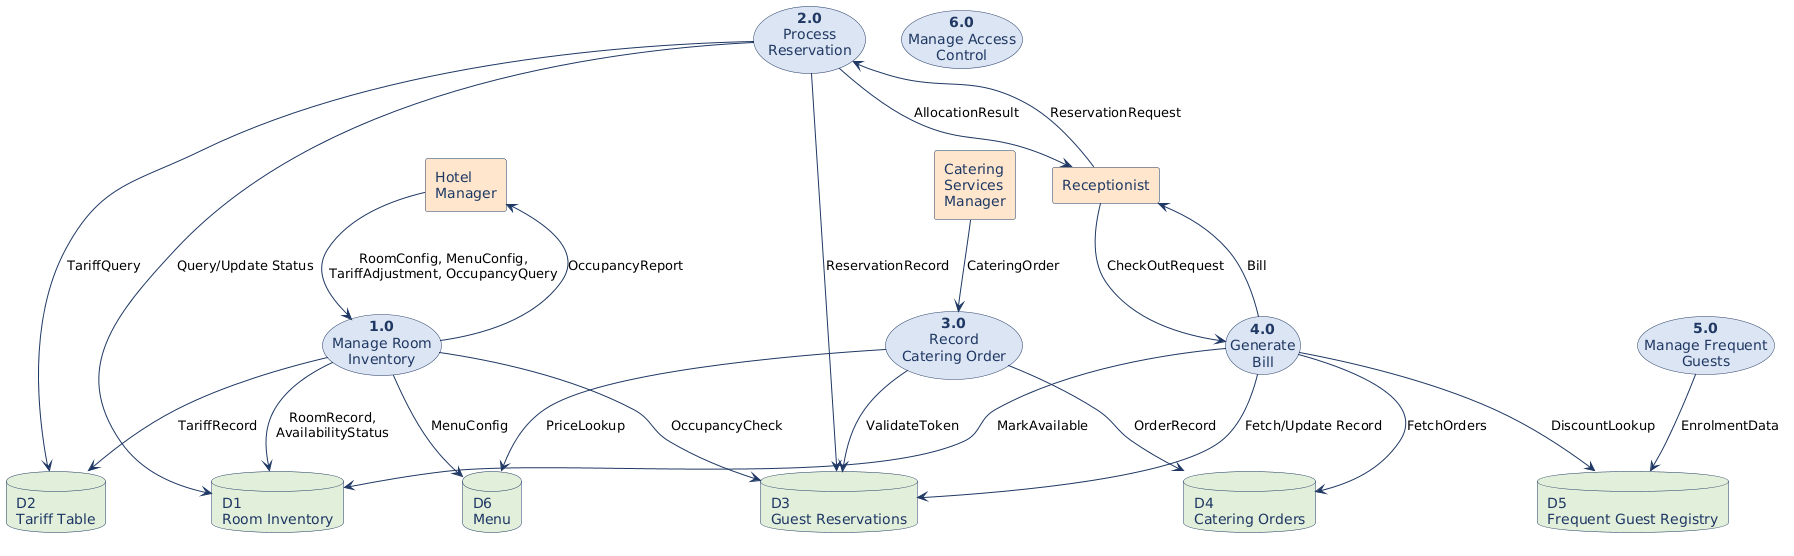
\includegraphics[width=\textwidth,keepaspectratio]{level1.png}
\caption{Level-1 DFD --- six cooperating processes and six data stores.}
\label{fig:level1}
\end{figure}

\subsubsection{Process Summaries}

\begin{longtable}{|L{1.2cm}|L{3.2cm}|L{6.5cm}|L{2.5cm}|}
  \hline
  \thead{ID} & \thead{Process} & \thead{Purpose} & \thead{SRS Ref} \\
  \hline
  \endhead
  \hline
  \endfoot
  \rowcolor{rowaltbg}
  1.0 & Manage Room Inventory
    & Accept room configuration and menu inputs from the Hotel Manager; validate and
      persist room records, tariffs, and food-item prices; compute and return the
      occupancy report for a given month; apply tariff revision requests.
    & FR-1.*, FR-2.*, FR-5.3, FR-8.7, FR-8.8 \\
  \hline
  2.0 & Process Reservation
    & Accept reservation requests from the Receptionist; check room availability for
      the requested type and dates; allocate a room and issue a token number, or
      generate an apology message if no suitable room is available. Exploded in
      \S\ref{sec:level2}.
    & FR-3.*, FR-4.*, FR-8.2--8.4 \\
  \hline
  \rowcolor{rowaltbg}
  3.0 & Record Catering Order
    & Accept catering orders from the Catering Services Manager; validate the token
      number against active guest records; persist the order against the guest's account
      for later billing.
    & FR-5.1--5.4 \\
  \hline
  4.0 & Generate Bill
    & On check-out request, retrieve the guest's room charge and accumulated catering
      charges; apply advance payment and any frequent-guest discount; produce and return
      an itemised bill; mark the room as available.
    & FR-6.1--6.6, FR-8.5--8.6 \\
  \hline
  \rowcolor{rowaltbg}
  5.0 & Manage Frequent Guests
    & Maintain the frequent-guest registry; validate loyalty identity numbers at
      reservation time; enrol new frequent guests; supply the applicable discount
      percentage to the billing process.
    & FR-7.1--7.4 \\
  \hline
  6.0 & Manage Access Control
    & Enforce role-based access: restrict panel visibility and operations to authorised
      user classes (Hotel Manager, Receptionist, Catering Services Manager).
    & NFR-S1, FR-8.1 \\
  \hline
\end{longtable}

\subsubsection{Data Store Summaries}

\begin{longtable}{|L{1.2cm}|L{3.2cm}|L{9.5cm}|}
  \hline
  \thead{ID} & \thead{Data Store} & \thead{Contents} \\
  \hline
  \endhead
  \hline
  \endfoot
  \rowcolor{rowaltbg}
  D1 & Room Inventory
    & Per-room records: room number, bed type, AC type, current availability status,
      and the tariff category applicable at check-in. \\
  \hline
  D2 & Tariff Table
    & Current and historical tariffs per room type (single-AC, single-Non-AC,
      double-AC, double-Non-AC), including the tariff change log (room type, old
      tariff, new tariff, date of change). \\
  \hline
  \rowcolor{rowaltbg}
  D3 & Guest Reservations
    & Per-reservation records: token number, guest name, room number, arrival
      date/time, approximate and actual check-out date/time, advance payment, and
      optional frequent-guest identity number. \\
  \hline
  D4 & Catering Orders
    & Per-order records: token number, food item name, quantity, unit price at time
      of order, date and time of consumption. \\
  \hline
  \rowcolor{rowaltbg}
  D5 & Frequent Guest Registry
    & Loyalty records: identity number, guest name, contact information, and the
      configured discount percentage. \\
  \hline
  D6 & Menu
    & Food and beverage items with current unit prices, configurable by the Hotel
      Manager. \\
  \hline
\end{longtable}

\newpage

\subsection{Level-2 DFD --- Explosion of 2.0 Process Reservation}
\label{sec:level2}

\begin{figure}[H]
\centering
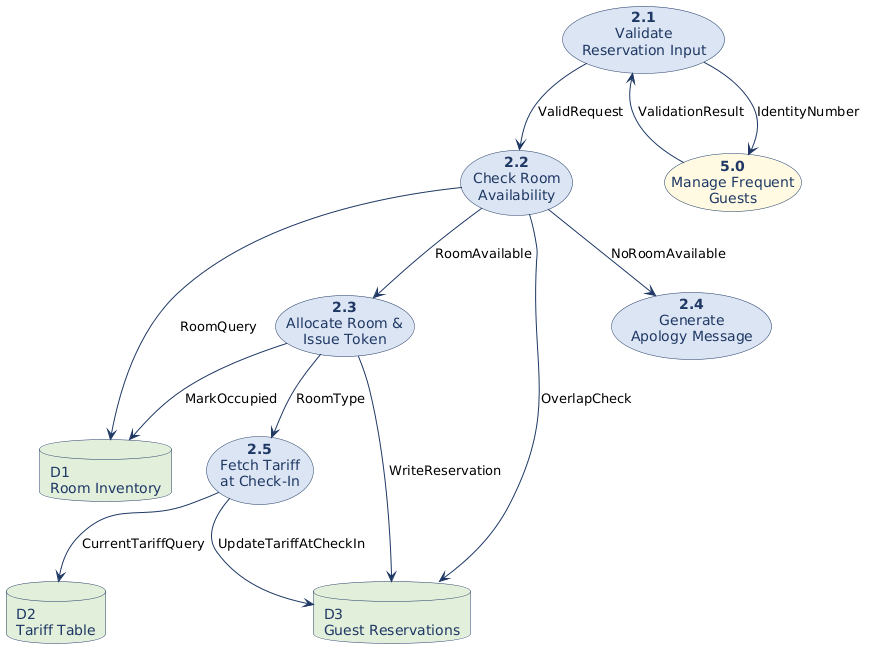
\includegraphics[width=\textwidth,keepaspectratio]{level2.png}
\caption{Level-2 DFD: explosion of \textbf{2.0 Process Reservation}. 5.0 Manage
Frequent Guests (shaded) is an upstream process from the Level-1 DFD consulted during
loyalty validation.}
\label{fig:level2}
\end{figure}

\subsubsection{Process Summaries (Level 2)}

\begin{longtable}{|L{1.2cm}|L{3.2cm}|L{9.5cm}|}
  \hline
  \thead{ID} & \thead{Process} & \thead{Purpose (SRS ref in brackets)} \\
  \hline
  \endhead
  \hline
  \endfoot
  \rowcolor{rowaltbg}
  2.1 & Validate Reservation Input
    & Accept raw reservation data from the Receptionist; check that all mandatory fields
      are non-empty and within valid ranges (arrival date not in the past, duration
      $\geq 1$ night, advance payment $\geq 0$); if a frequent-guest identity number is
      supplied, delegate validation to 5.0. [FR-3.1, FR-3.2, FR-8.9] \\
  \hline
  2.2 & Check Room Availability
    & Query D1 to find rooms matching the requested bed type and AC type that are not
      occupied for the requested date range; return the first available room number
      (lowest room number), or a \texttt{NoRoomAvailable} flag. [FR-4.1, NFR-R3] \\
  \hline
  \rowcolor{rowaltbg}
  2.3 & Allocate Room \& Issue Token
    & If a room is available, mark it \texttt{occupied} in D1 for the reservation
      period; generate a unique token number; write the reservation record to D3; return
      the room number and token number to the Receptionist. [FR-4.2, FR-4.4] \\
  \hline
  2.4 & Generate Apology Message
    & If no suitable room is available, compose an apology message stating the
      unavailability and the reason (no room of the requested type on the requested
      dates) and return it to the Receptionist. [FR-4.3] \\
  \hline
  \rowcolor{rowaltbg}
  2.5 & Fetch Tariff at Check-In
    & Retrieve the current tariff for the allocated room type from D2 and record it
      in the reservation entry in D3, so that billing uses the tariff prevailing at
      check-in time rather than the tariff at check-out time. [FR-6.2] \\
  \hline
\end{longtable}

\newpage

% ══════════════════════════════════════════════════════════════════════════════
\subsection{Data Dictionary}
\label{sec:datadict}

The data dictionary uses the standard structured-analysis notation:
\texttt{=} (is composed of), \texttt{+} (and), \texttt{[\,|\,]} (either-or),
\texttt{\{\,\}} (iteration), \texttt{(\,)} (optional), \texttt{**} (comment).

\begin{longtable}{|L{3.8cm}|L{10cm}|}
  \hline
  \thead{Name} & \thead{Definition} \\
  \hline
  \endhead
  \hline
  \endfoot
  \rowcolor{rowaltbg}
  \texttt{RoomConfig}
    & = \{RoomRecord\} \newline
      \texttt{RoomRecord} = RoomNumber + BedType + ACType \newline
      \texttt{BedType} = [ \texttt{Single} | \texttt{Double} ] \newline
      \texttt{ACType} = [ \texttt{AC} | \texttt{Non-AC} ] \\
  \hline
  \texttt{TariffAdjustment}
    & = RoomType + AdjustmentPct \qquad
      ** $-100 < \text{AdjustmentPct}$; positive = upward revision ** \\
  \hline
  \rowcolor{rowaltbg}
  \texttt{OccupancyQuery}
    & = MonthYear \qquad ** format YYYY-MM ** \\
  \hline
  \texttt{OccupancyReport}
    & = MonthYear + TotalRoomNightsAvailable + TotalRoomNightsOccupied
        + AverageOccupancyPct \\
  \hline
  \rowcolor{rowaltbg}
  \texttt{MenuConfig}
    & = \{FoodItemRecord\} \newline
      \texttt{FoodItemRecord} = FoodItemName + UnitPrice \\
  \hline
  \texttt{ReservationRequest}
    & = GuestName + ArrivalDateTime + ApproxDurationNights + RoomTypePreference
        + AdvancePaid + (IdentityNumber) \newline
      \texttt{RoomTypePreference} = BedType + ACType \\
  \hline
  \rowcolor{rowaltbg}
  \texttt{AllocationResult}
    & = [ SuccessResult | ApologyMessage ] \newline
      \texttt{SuccessResult} = RoomNumber + TokenNumber \newline
      \texttt{ApologyMessage} = WarningText + UnavailableRoomType + RequestedDates \\
  \hline
  \texttt{CateringOrder}
    & = TokenNumber + FoodItemName + Quantity + OrderDateTime \\
  \hline
  \rowcolor{rowaltbg}
  \texttt{CheckOutRequest}
    & = TokenNumber \\
  \hline
  \texttt{Bill}
    & = GuestName + RoomNumber + TokenNumber + CheckInDateTime + CheckOutDateTime
        + \{RoomChargeLineItem\} + \{CateringLineItem\} + TotalBillAmount
        + AdvancePaidDeducted + (DiscountDeducted) + NetBalancePayable \newline
      \texttt{RoomChargeLineItem} = TariffPerNight + ActualNightsStayed
        + RoomChargeSubtotal \newline
      \texttt{CateringLineItem} = FoodItemName + Quantity + UnitPrice
        + CateringSubtotal \\
  \hline
  \rowcolor{rowaltbg}
  \texttt{RoomRecord}
    & = RoomNumber + BedType + ACType
        + [ \texttt{available} | \texttt{occupied} ] \\
  \hline
  \texttt{TariffRecord}
    & = RoomType + CurrentTariff + \{TariffChangeEntry\} \newline
      \texttt{TariffChangeEntry} = OldTariff + NewTariff + ChangeDate \\
  \hline
  \rowcolor{rowaltbg}
  \texttt{ReservationRecord}
    & = TokenNumber + GuestName + RoomNumber + RoomType + TariffAtCheckIn
        + ArrivalDateTime + ApproxDurationNights + (ActualCheckOutDateTime)
        + AdvancePaid + (IdentityNumber) \\
  \hline
  \texttt{CateringOrderRecord}
    & = TokenNumber + FoodItemName + Quantity + UnitPrice + OrderDateTime \\
  \hline
  \rowcolor{rowaltbg}
  \texttt{FrequentGuestRecord}
    & = IdentityNumber + GuestName + ContactInfo + DiscountPct \\
  \hline
  \texttt{TokenNumber}
    & = Integer \qquad ** system-generated, unique across lifetime of DB ** \\
  \hline
\end{longtable}

\newpage

% ══════════════════════════════════════════════════════════════════════════════
\section{Structured Design}

\subsection{Design Strategy}

The Level-1 DFD exhibits a classical \textbf{transaction-centred} shape: afferent flows
(\texttt{ReservationRequest}, \texttt{CateringOrder}, \texttt{CheckOutRequest},
\texttt{TariffAdjustment}, \texttt{OccupancyQuery}) arrive at a transaction centre
which dispatches each transaction to one of several dedicated action branches
(Reservation, Catering, Billing, Room Management, Frequent-Guest Management). We
therefore apply \textbf{transaction analysis} to derive the structure chart: one root
coordinator with a transaction dispatcher and one sub-tree per transaction type, plus
shared utility modules for database access and input validation.

\subsection{Structure Chart}

\begin{figure}[H]
\centering
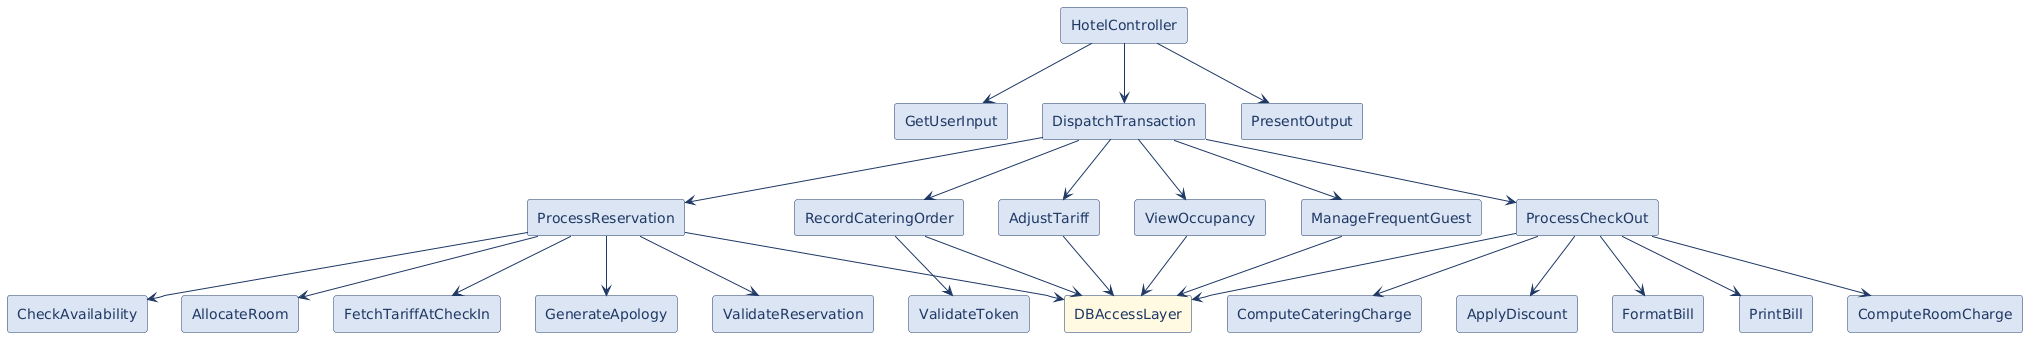
\includegraphics[width=\textwidth,keepaspectratio]{structchart.png}
\caption{Structure Chart (transaction-analysis derived). \texttt{DBAccessLayer}
(shaded) is a shared utility module invoked across all transaction branches. Data /
flag couples are listed in Table~\ref{tbl:couples}.}
\label{fig:structchart}
\end{figure}

\subsubsection{Data and Flag Couples}
\label{tbl:couples}

The following couples annotate the calls in Figure~\ref{fig:structchart}. ``Down'' =
caller $\to$ callee, ``Up'' = callee $\to$ caller.

\begin{longtable}{|L{3cm}|L{3cm}|L{3cm}|L{4.5cm}|}
  \hline
  \thead{Caller} & \thead{Callee} & \thead{Couple} & \thead{Payload} \\
  \hline
  \endhead
  \hline
  \endfoot
  \rowcolor{rowaltbg}
  HotelController      & GetUserInput         & data (up)   & TransactionRequest \\
  \hline
  HotelController      & Dispatch-Transaction  & data (down) & TransactionRequest \\
  \hline
  \rowcolor{rowaltbg}
  HotelController      & PresentOutput        & data (down) & TransactionResult \\
  \hline
  Dispatch-Transaction  & Process-Reservation   & data (down) \newline data (up)
                                                  & ReservationRequest \newline AllocationResult \\
  \hline
  \rowcolor{rowaltbg}
  Dispatch-Transaction  & Record-CateringOrder  & data (down) \newline flag (up)
                                                  & CateringOrder \newline OrderOkFlag \\
  \hline
  Dispatch-Transaction  & ProcessCheckOut      & data (down) \newline data (up)
                                                  & CheckOutRequest \newline Bill \\
  \hline
  \rowcolor{rowaltbg}
  Dispatch-Transaction  & AdjustTariff         & data (down) \newline flag (up)
                                                  & TariffAdjustment \newline AdjustOkFlag \\
  \hline
  Dispatch-Transaction  & ViewOccupancy        & data (down) \newline data (up)
                                                  & OccupancyQuery \newline OccupancyReport \\
  \hline
  \rowcolor{rowaltbg}
  Process-Reservation   & Validate-Reservation  & data (down) \newline flag (up)
                                                  & ReservationRequest \newline ValidFlag, ErrorList \\
  \hline
  Process-Reservation   & CheckAvailability    & data (down) \newline data (up)
                                                  & RoomTypePreference, DateRange \newline RoomNumber or \texttt{null} \\
  \hline
  \rowcolor{rowaltbg}
  Process-Reservation   & AllocateRoom         & data (down) \newline data (up)
                                                  & ReservationRequest, RoomNumber \newline TokenNumber \\
  \hline
  Process-Reservation   & GenerateApology      & data (down) \newline data (up)
                                                  & RoomTypePreference, DateRange \newline ApologyMessage \\
  \hline
  \rowcolor{rowaltbg}
  ProcessCheckOut      & Compute-RoomCharge    & data (down) \newline data (up)
                                                  & ReservationRecord \newline RoomChargeSubtotal \\
  \hline
  ProcessCheckOut      & Compute-CateringCharge & data (down) \newline data (up)
                                                  & TokenNumber \newline CateringChargeSubtotal \\
  \hline
  \rowcolor{rowaltbg}
  ProcessCheckOut      & ApplyDiscount        & data (down) \newline data (up)
                                                  & IdentityNumber, TotalCharge \newline DiscountAmt \\
  \hline
  ProcessCheckOut      & FormatBill           & data (down) \newline data (up)
                                                  & BillComponents \newline Bill \\
  \hline
  \rowcolor{rowaltbg}
  Record-CateringOrder  & ValidateToken        & data (down) \newline flag (up)
                                                  & TokenNumber \newline ActiveFlag \\
  \hline
  $*$ (all branches)   & DBAccessLayer        & data (down) \newline data (up)
                                                  & Query / WriteRequest \newline ResultSet or \texttt{null} \\
  \hline
\end{longtable}

\noindent\textbf{Coupling / cohesion.}
\begin{itemize}[leftmargin=1.5em]
  \item All data couples are \emph{simple data} (no tramp data); no global state is
        shared between modules other than through the database access layer.
  \item \texttt{ValidFlag}, \texttt{OrderOkFlag}, \texttt{AdjustOkFlag}, and
        \texttt{ActiveFlag} are control couples; each encodes a single binary outcome
        and justifies its role as a genuine control signal.
  \item Every leaf module exhibits \textbf{functional cohesion} (one well-defined job).
  \item The \texttt{Process-Reservation} and \texttt{ProcessCheckOut} modules are
        \textbf{sequential cohesive}: each step feeds the next in a well-defined pipeline.
  \item \texttt{DBAccessLayer} is a \textbf{communicational cohesion} shared-service
        module whose sole responsibility is mediated database I/O, keeping all other
        modules database-agnostic.
\end{itemize}

\newpage

% ══════════════════════════════════════════════════════════════════════════════
\subsection{Module Specifications}

Each module is specified as \textbf{(Inputs | Outputs | Processing)}.

\begin{longtable}{|L{3.2cm}|L{10.5cm}|}
  \hline
  \thead{Module} & \thead{Specification (SRS ref)} \\
  \hline
  \endhead
  \hline
  \endfoot
  \rowcolor{rowaltbg}
  \texttt{HotelController}
    & \textbf{In:} GUI events from all user classes. \textbf{Out:} lifecycle transitions,
      displayed results.
      \textbf{Proc:} Top-level coordinator. Authenticates the active user class, enables
      or disables panels per role (NFR-S1). Sequences
      \texttt{GetUserInput $\to$ Dispatch-Transaction $\to$ PresentOutput} for each
      user action. Runs background database tasks on a worker thread to preserve GUI
      responsiveness (NFR-P3). [FR-8.1, NFR-S1] \\
  \hline
  \texttt{GetUserInput}
    & \textbf{In:} Swing form field values and button events. \textbf{Out:}
      \texttt{TransactionRequest} (typed DTO).
      \textbf{Proc:} Pulls values from the active form panel into a typed DTO;
      determines the transaction type (reservation, catering, check-out, tariff
      adjustment, occupancy query, frequent-guest enrolment). [FR-8.2--8.10] \\
  \hline
  \rowcolor{rowaltbg}
  \texttt{Dispatch-
  Transaction}
    & \textbf{In:} \texttt{TransactionRequest}. \textbf{Out:} \texttt{TransactionResult}.
      \textbf{Proc:} \texttt{switch} on transaction type; delegates to
      \texttt{Process-Reservation}, \texttt{Record-CateringOrder},
      \texttt{ProcessCheckOut}, \texttt{AdjustTariff}, \texttt{ViewOccupancy}, or
      \texttt{ManageFrequentGuest}. \\
  \hline
  \texttt{PresentOutput}
    & \textbf{In:} \texttt{TransactionResult}. \textbf{Out:} rendered GUI panel / dialog.
      \textbf{Proc:} Formats and displays the result in the appropriate output panel;
      invokes \texttt{PrintBill} if the result is a \texttt{Bill} and the user confirms
      printing. [FR-8.5, FR-8.6] \\
  \hline
  \rowcolor{rowaltbg}
  \texttt{Process-
  Reservation}
    & \textbf{In:} \texttt{ReservationRequest}. \textbf{Out:} \texttt{AllocationResult}.
      \textbf{Proc:} Orchestrates \texttt{Validate-Reservation $\to$ CheckAvailability};
      if available, calls \texttt{AllocateRoom} and \texttt{FetchTariffAtCheckIn};
      otherwise calls \texttt{GenerateApology}. [FR-3.*, FR-4.*] \\
  \hline
  \texttt{Validate-
  Reservation}
    & \textbf{In:} \texttt{ReservationRequest}. \textbf{Out:} \texttt{ValidFlag},
      \texttt{ErrorList}.
      \textbf{Proc:} Checks mandatory fields, date validity, duration $\geq 1$,
      advance payment $\geq 0$; if \texttt{IdentityNumber} present, calls
      \texttt{LookupFrequentGuest} to confirm it exists. [FR-3.1, FR-8.9] \\
  \hline
  \rowcolor{rowaltbg}
  \texttt{Check-
  Availability}
    & \textbf{In:} \texttt{RoomTypePreference}, \texttt{DateRange}.
      \textbf{Out:} lowest available \texttt{RoomNumber} or \texttt{null}.
      \textbf{Proc:} Queries D1 via \texttt{DBAccessLayer} for rooms of the requested
      type; filters out rooms with overlapping active reservations from D3;
      returns the lowest-numbered match. [FR-4.1, NFR-R3] \\
  \hline
  \texttt{AllocateRoom}
    & \textbf{In:} \texttt{ReservationRequest}, \texttt{RoomNumber}.
      \textbf{Out:} \texttt{TokenNumber}.
      \textbf{Proc:} Generates a unique \texttt{TokenNumber} (auto-increment primary
      key); writes the reservation record to D3 via \texttt{DBAccessLayer}; marks the
      room \texttt{occupied} in D1 for the reservation period. [FR-4.2, FR-4.4] \\
  \hline
  \rowcolor{rowaltbg}
  \texttt{FetchTariff-
  AtCheckIn}
    & \textbf{In:} \texttt{RoomType}. \textbf{Out:} \texttt{TariffAtCheckIn}.
      \textbf{Proc:} Reads the current tariff for the room type from D2 via
      \texttt{DBAccessLayer} and stores it in the reservation record so that billing
      is insulated from future tariff changes. [FR-6.2] \\
  \hline
  \texttt{GenerateApology}
    & \textbf{In:} \texttt{RoomTypePreference}, \texttt{DateRange}.
      \textbf{Out:} \texttt{ApologyMessage}.
      \textbf{Proc:} Composes a message stating the requested type and dates for which
      no room is available. [FR-4.3] \\
  \hline
  \rowcolor{rowaltbg}
  \texttt{Record-
  CateringOrder}
    & \textbf{In:} \texttt{CateringOrder}. \textbf{Out:} \texttt{OrderOkFlag}.
      \textbf{Proc:} Calls \texttt{ValidateToken}; if valid, looks up the unit price of
      the food item from D6 via \texttt{DBAccessLayer}; writes the order record to D4.
      [FR-5.1--5.4] \\
  \hline
  \texttt{ValidateToken}
    & \textbf{In:} \texttt{TokenNumber}. \textbf{Out:} \texttt{ActiveFlag}.
      \textbf{Proc:} Queries D3 via \texttt{DBAccessLayer} to confirm the token
      corresponds to a currently checked-in guest (arrival $\leq$ now and no
      \texttt{ActualCheckOutDateTime} recorded). [FR-5.2] \\
  \hline
  \rowcolor{rowaltbg}
  \texttt{ProcessCheckOut}
    & \textbf{In:} \texttt{CheckOutRequest} (token number). \textbf{Out:} \texttt{Bill}.
      \textbf{Proc:} Retrieves reservation record from D3; calls
      \texttt{ComputeRoom-Charge}, \texttt{ComputeCater-Charge}, and optionally
      \texttt{ApplyDiscount}; calls \texttt{FormatBill}; records actual check-out
      date/time in D3; marks room \texttt{available} in D1. [FR-6.1--6.6] \\
  \hline
  \texttt{Compute-
  RoomCharge}
    & \textbf{In:} \texttt{ReservationRecord}. \textbf{Out:} \texttt{RoomChargeSubtotal}.
      \textbf{Proc:} $\text{RoomCharge} = \text{TariffAtCheckIn} \times
      \lceil(\text{CheckOut} - \text{CheckIn})/24\text{h}\rceil$.
      Rounds to two decimal places. [FR-6.2, NFR-R4] \\
  \hline
  \rowcolor{rowaltbg}
  \texttt{Compute-
  CateringCharge}
    & \textbf{In:} \texttt{TokenNumber}. \textbf{Out:} \{CateringLineItem\}, \texttt{CateringChargeSubtotal}.
      \textbf{Proc:} Retrieves all catering orders for the token from D4;
      $\text{CateringCharge} = \sum (\text{Quantity}_i \times \text{UnitPrice}_i)$.
      Rounds to two decimal places. [FR-6.3, NFR-R4] \\
  \hline
  \texttt{ApplyDiscount}
    & \textbf{In:} \texttt{IdentityNumber}, \texttt{TotalCharge}.
      \textbf{Out:} \texttt{DiscountAmt}.
      \textbf{Proc:} Looks up \texttt{DiscountPct} for the identity number in D5 via
      \texttt{DBAccessLayer};
      $\text{DiscountAmt} = \text{TotalCharge} \times \text{DiscountPct} / 100$.
      [FR-7.3, NFR-R4] \\
  \hline
  \rowcolor{rowaltbg}
  \texttt{FormatBill}
    & \textbf{In:} \texttt{BillComponents} (reservation record, line items, charges,
      discount, advance paid). \textbf{Out:} \texttt{Bill}.
      \textbf{Proc:} Assembles the itemised bill DTO per FR-6.4;
      $\text{NetBalance} = \text{TotalCharge} - \text{DiscountAmt} - \text{AdvancePaid}$.
      Two-decimal rounding throughout. [FR-6.4, NFR-R4] \\
  \hline
  \texttt{PrintBill}
    & \textbf{In:} \texttt{Bill}. \textbf{Out:} print job.
      \textbf{Proc:} Formats the bill as a printable layout and submits to the Java
      \texttt{PrinterJob} API targeting the system's default printer. [FR-6.5] \\
  \hline
  \rowcolor{rowaltbg}
  \texttt{AdjustTariff}
    & \textbf{In:} \texttt{TariffAdjustment}. \textbf{Out:} \texttt{AdjustOkFlag}.
      \textbf{Proc:} Reads current tariff from D2; computes
      $\text{NewTariff} = \text{CurrentTariff} \times (1 + \text{AdjPct}/100)$;
      writes new tariff and appends a \texttt{TariffChangeEntry} to D2 via
      \texttt{DBAccessLayer}. [FR-2.2, FR-2.3] \\
  \hline
  \texttt{ViewOccupancy}
    & \textbf{In:} \texttt{OccupancyQuery}. \textbf{Out:} \texttt{OccupancyReport}.
      \textbf{Proc:} Queries D3 for all reservations overlapping the selected month;
      computes \texttt{TotalRoomNightsOccupied} and \texttt{TotalRoomNightsAvailable}
      from D1; calculates \texttt{AverageOccupancyPct}. [FR-2.1] \\
  \hline
  \rowcolor{rowaltbg}
  \texttt{Manage-
  FrequentGuest}
    & \textbf{In:} enrolment data or lookup request. \textbf{Out:} \texttt{IdentityNumber}
      (enrolment) or \texttt{FrequentGuestRecord} (lookup).
      \textbf{Proc:} On enrolment, generates a new \texttt{IdentityNumber} and writes
      to D5; on lookup, retrieves record from D5 by identity number and returns the
      discount percentage. [FR-7.1, FR-7.2, FR-7.4] \\
  \hline
  \texttt{Lookup-
  FrequentGuest}
    & \textbf{In:} \texttt{IdentityNumber}. \textbf{Out:} \texttt{ValidFlag},
      \texttt{DiscountPct}.
      \textbf{Proc:} Queries D5 via \texttt{DBAccessLayer}; returns \texttt{true} and
      discount if found, \texttt{false} otherwise. [FR-7.3] \\
  \hline
  \rowcolor{rowaltbg}
  \texttt{DBAccessLayer}
    & \textbf{In:} typed query or write request. \textbf{Out:} \texttt{ResultSet} or
      \texttt{null}.
      \textbf{Proc:} Single-responsibility database gateway. Translates typed DTOs
      into parameterised SQL statements; executes against the embedded RDBMS; maps
      result rows back to typed objects. All transactional commits are performed here.
      No business logic resides in this module. [NFR-R5] \\
  \hline
\end{longtable}

\newpage

% ══════════════════════════════════════════════════════════════════════════════
\section{Requirements Traceability}
\label{sec:trace}

\begin{longtable}{|L{3cm}|L{3.5cm}|L{3cm}|L{4cm}|}
  \hline
  \thead{SRS Req.\ ID} & \thead{DFD Process} & \thead{Data Store} & \thead{Structure-chart Module} \\
  \hline
  \endhead
  \hline
  \endfoot
  \rowcolor{rowaltbg}
  FR-1.1 -- FR-1.3 & 1.0 & D1 & DBAccessLayer (room writes) \\
  \hline
  FR-2.1           & 1.0, 6.0 & D1, D3 & ViewOccupancy \\
  \hline
  \rowcolor{rowaltbg}
  FR-2.2 -- FR-2.3 & 1.0 & D2 & AdjustTariff \\
  \hline
  FR-3.1 -- FR-3.2 & 2.0, 2.1 & --- & Validate-Reservation \\
  \hline
  \rowcolor{rowaltbg}
  FR-4.1           & 2.2 & D1, D3 & CheckAvailability \\
  \hline
  FR-4.2, FR-4.4   & 2.3 & D1, D3 & AllocateRoom \\
  \hline
  \rowcolor{rowaltbg}
  FR-4.3           & 2.4 & --- & GenerateApology \\
  \hline
  FR-5.1 -- FR-5.4 & 3.0 & D4, D6 & Record-CateringOrder, ValidateToken \\
  \hline
  \rowcolor{rowaltbg}
  FR-5.3           & 1.0 & D6 & DBAccessLayer (menu writes) \\
  \hline
  FR-6.1 -- FR-6.4 & 4.0 & D3, D4 & ProcessCheckOut, ComputeRoom-Charge, ComputeCater-Charge, FormatBill \\
  \hline
  \rowcolor{rowaltbg}
  FR-6.2           & 2.5 & D2, D3 & FetchTariffAtCheckIn \\
  \hline
  FR-6.5           & 4.0 & --- & PrintBill \\
  \hline
  \rowcolor{rowaltbg}
  FR-6.6           & 4.0 & D1 & ProcessCheckOut (room release) \\
  \hline
  FR-7.1 -- FR-7.2 & 5.0 & D5 & ManageFrequentGuest \\
  \hline
  \rowcolor{rowaltbg}
  FR-7.3           & 5.0, 4.0 & D5 & LookupFrequentGuest, ApplyDiscount \\
  \hline
  FR-7.4           & 5.0 & D5 & ManageFrequentGuest (enrolment) \\
  \hline
  \rowcolor{rowaltbg}
  FR-8.1 -- FR-8.10 & 1.0, 2.0, 4.0, 5.0, 6.0 & --- & HotelController, GetUserInput, PresentOutput \\
  \hline
  NFR-P3           & --- & --- & HotelController (background thread) \\
  \hline
  \rowcolor{rowaltbg}
  NFR-R3           & 2.2 & D1, D3 & CheckAvailability (overlap check) \\
  \hline
  NFR-R4           & 4.0 & --- & ComputeRoom-Charge, ComputeCater-Charge, ApplyDiscount, FormatBill \\
  \hline
  \rowcolor{rowaltbg}
  NFR-R5           & --- & D1--D6 & DBAccessLayer (transactional commits) \\
  \hline
  NFR-S1           & 6.0 & --- & HotelController (role-based panel control) \\
  \hline
\end{longtable}

% ══════════════════════════════════════════════════════════════════════════════
\section{Revision History}

\begin{longtable}{|L{2cm}|L{3cm}|L{4cm}|L{4.5cm}|}
  \hline
  \thead{Version} & \thead{Date} & \thead{Author} & \thead{Description} \\
  \hline
  \endhead
  \hline
  \endfoot
  \rowcolor{rowaltbg}
  1.0 & \today & Project Team
    & Initial SA/SD for Hotel Automation Software. Context diagram, Level-1 DFD
      (six processes, six data stores), Level-2 explosion of Process Reservation,
      data dictionary, transaction-analysis-derived structure chart with module
      specifications, and full traceability matrix. Based on SRS\_HotelAutomation. \\
  \hline
\end{longtable}

\vfill
\begin{center}
  \color{medblue}\rule{0.6\linewidth}{0.5pt}\\[0.5em]
  \color{gray}\small\textit{End of Document --- Hotel Automation Software SA/SD v1.0}
\end{center}

\end{document}